\chapter{Collider Physics and Phenomenology}

\section{Introduction}

In the previous chapter, we outlined how we reach a theory like the standard model from fundamental principles, but 
a considerable amount of physics is required to reach a practical theoretical description of what occurs inside of 
the experiment. The goal of this section is to connect the matrix elements $\mathcal{M}$ from the quantum field
theoretic description  of the Standard Model to the Monte Carlo simulations used to test a given theory. 
First, we will discuss the how
we can compare the matrix amplitudes with the observations in a physical detector. After, we will the discuss the considerations 
that must be made for the fact the LHC collides hadrons rather than fundamental particles. Finally, we will discuss the framework used to describe the particles actually observed in the detector after the hard scattering occurs where perturbative physics breaks down and  calculations from first principles cannot be performed. Generic principles for parton showering and hadronization mdoels will be examined. 

\section{From Matrix Elements to Cross Sections} 

In high energy experimental particle physics the key quantity (besides particle quantum numbers and masses) is the
cross section $\sigma$ of the process. This is the rate or in essence, the probability that an event occurs. It is the proportionality between the number of observed collisions and the rate at which the Large Hadron Collider delivers collsions $L$ (the luminosity)
 expressed simply as:
\begin{align*}
N_{events} = L \times \sigma
\end{align*}
cite-peskin
Consider a target of particles type $A$ and density $\rho_A$ and aim particles type 
$B$ with density $\rho_B$. If the lengths of the bunches of particles are $l_A$ and $l_B$ 
then the cross section of the processes is defined for a beam with cross-sectional area as:
\begin{align*}
\sigma \equiv \frac{N_{events}}{\rho_A l_A \rho_B l_B A}
\end{align*}
Inverting this and assuming that we have constant density along the beams length:
\begin{equation}\label{eq:sigma}
N_{events} = \frac{\sigma N_A N_B}{A} = \sigma{N_A n_B}
\end{equation}
by comparing this with the relation for $N_{events}$ above containing luminosity, we see the
 luminosity is in effect counting the number of colliding particles per unit area.
 More incident particles and a more focused beam means more scattered events. 
In the last equality we have introduced the impact parameter density $n_B$ for
 the incident $B$ particles.

However, the the end results of feynman diagram calculations yield scattering amplitudes
which are matrix elements of scattering a given intial state into a given final state, not
a cross section. We have to further develop the stocastic interaction of two particles into
something more concrete experimentally.
 
First, we need  must think about the quantum fields within the beams that are colliding. To do so we set up two initial 
wave packets $A$ and $B$ in a limit of definite momentum $p_A$ and $p_B$ and evolve them for a very long time 
with the time evolution operator $\exp{(-iHt)}$ and then consider the final state wave packets with the correct final state particles. This in turn will give us the probability amplitude for producing that final state.  
\begin{align*}
\mathcal{P} = |\langle \phi_1 \phi_2 \ldots| \phi_A \phi_B \rangle | ^2 
\end{align*}
Now consider the number of incident particles colliding along the z-axis, but with non-trivial transverse displacement,
also referred to as impact parameters $b_i$. We will take the perspective that $A$ is a target and $B$ is collinear
with the target and account for the shift in position with an explict factor of $\exp(-ib \cdot k_B)$. The properly normalized expression then reads:  
\begin{align*}
|\phi_A \phi_B \rangle = \int \frac{d^3k_A}{\sqrt{2E_A}(2\pi)^3} \int \frac{d^3k_B}{\sqrt{2E_B}(2\pi)^3}\phi_A(k_A)\phi_B(k_B) e^{-ib \cdot k_B} 
\end{align*}
For a single target $A$ and a beam $B$ with with constant impact parameter density $n_B = N_B / A$ we can write the the number of events as
\begin{align*}
N_{events} = \sum_{\text{incident particles } i} \mathcal{P}_i = \int d^2b n_B(b) \mathcal{P}(b) = n_B \int d^2b \mathcal{P}(b) 
\end{align*}
Comparing this to Equation \ref{eq:sigma} we can write the cross section as:
\begin{align*}
\sigma = \int d^2 b \mathcal{P}(b) 
\end{align*}
and the properly normalized differential cross section for scattering into a the infinitesimal final state momentum element is:
\begin{align*}
 d\sigma &= \left( \prod_f \frac{d^3p_f}{(2\pi)^3 2E_f} \right ) \int d^2b \left ( \prod_{i=A,B}
 \int \frac{d^3 k_i }{(2\pi)^3 \sqrt{2E_i}} \phi_i(k_i) \int \frac{d^3 \bar{k}_i}{(2\pi)^3
\sqrt{2\bar{E}_i}} \phi^*_i(\bar{k}_i) \right)\\ 
 &\times e^{ib\cdot (\bar{k}_S - k_B)} | \langle \{ p_f\} | \{k_i \} \rangle |^2 
\end{align*}
We have 6 dummy integrals to do in $\bar{k}$ over the 3 momentums of particle $A$ and $B$
 so count our delta functions. The $d^2b$ integral gives 2 delta functions in the transverse 
momentum $(2\pi)^2 \delta^2(k_B^\perp - \bar{k}_B^\perp)$.  We have 8 delta functions from 
the matrix element enforcing that the process to conserve energy and momentum
 $\delta^4(k_A +k_B - \sum p_f)$\ and in the complex conjugate with the dummy variable
 $\bar{k}$: $\delta^4(\bar{k}_A + \bar{k}_B - \sum p_f)$. Performing the transverse 
integrals in $\bar{k}_B$ sets $\bar{k}_B^T=k_B^T$ which in combination with the transverse
 barred ampltidue delta functions give $\bar{k}_A^T = k_A^T$. The remaining 2 integrals in $z$ require some properties of delta functions:
\begin{align*}
\int d \bar{k}_A^z d \bar{k}_B^z \delta( \bar{k}^z_A + \bar{k}^z_B  - \sum p_f^z) \delta (\bar{E}_A + \bar{E}_B - \sum E_f) 
\end{align*}
We can integrate the first $B$ integral considering $\bar{k}_B^z$ to be a function of
$\bar{k}_A^z$ and writing the barred energy terms in the momentums and masses:
\begin{align*}
\int d\bar{k}_A^z  \delta \left (\sqrt{\bar{k}_A^2 +m_A^2}  + \sqrt{\bar{k}_B^2 + m_B^2} - \sum E_f \right) 
\end{align*}
We now need to use the property that $\delta[f(x)] = \sum_i (\delta(x_i) / f'(x_i))$ where $x_i$ are the zeros of the fuction $f(x)$. Note that given our parmeterization from the first delta function $\partial_{\bar{k}_A^z}(\bar{k}_B^2) = - 2 \bar{k}_B^z$.
\begin{align*}
&\int d\bar{k}_A^z  \left (\frac{1}{2} \frac{2\bar{k}_A}{\sqrt{\bar{k}_A^2 +m_A^2}}
 - \frac{1}{2} \frac{2\bar{k}_B}{\sqrt{\bar{k}_B^2 +m_B^2}} \right )^{-1}\delta(\bar{E}_A
 + \bar{E}_B - \sum E_f) \\
= &\frac{1}{\frac{\bar{k}_A}{\bar{E}_A}- \frac{\bar{k}_B}{\bar{E}_B}}
 \delta(\bar{E}_A + \bar{E}_B - \sum E_f) = \frac{1}{\beta_A - \beta_B}
\end{align*}
The 6 remaining integrals in $k_A$ and $k_B$ remain:
\begin{align*}
d\sigma &= \left( \prod_f \frac{d^3p_f}{(2\pi)^3 2E_f} \right ) \frac{|\mathcal{M}|^2}{2E_A2E_B|\beta_A - \beta_B|}
 \int \frac{d^3 k_A }{(2\pi)^3 \sqrt{2E_i}} |\phi_A(k_A)|^2 \\ 
&\times  \int \frac{d^3 k_B }{(2\pi)^3 \sqrt{2E_i}} |\phi_B(k_b)|^2 \delta^4( k_A + k_B - \sum p_f)
\end{align*}
To proceed further, we must consider the quality of measurements made by particle detectors. 
Real detectors cannot measure arbitrarily small spreads in the momentums $k_A+k_B$. 
The measurements made in a realistic experimental setup are not senitive to the
spread of momentum in the initial wave packets $\phi_A$ and $\phi_B$. Given this, we can take the central value $k_A+k_B=p_A+p_B$
to be a good approximation for the delta function. With this approximation, we can move the delta function outside the integral and
perform the integrals using the unit normalization condition of the two fields $\phi_i$:
\begin{equation} \label{eq:dsigma}
d\sigma = \left( \prod_f \frac{d^3p_f}{(2\pi)^3 2E_f} \right ) \frac{|\mathcal{M}|^2}{2E_A2E_B|\beta_A - \beta_B|} (2\pi)^4
\delta^4 \left (p_A+p_B - \sum p_f  \right )
\end{equation}
Let's consider the simple case of $2 \rightarrow 2$ scattering and use the energy delta function 
of the 4 remaining delta functions to compute integral over the final state.
To do so, we go to the center of mass frame where $|p_1| = |p_2|= P$, $\vec p_1 = - \vec p_2$, $E_{cm} = 2P$. We first
integrate $p_2$ to invorce 3-momentum conservation  
\begin{align*}
\int \left( \frac{d^3p_1}{(2\pi)^3 2E_1} \right )\left( \frac{d^3p_2}{(2\pi)^3 2E_2} \right )  (2\pi)^4 \delta^4( P - \sum p_f ) 
\end{align*}
now switching to a spherical integral with a jacobian $p_1^2 dp_1 d\Omega$ where $d\Omega$ is and infinitesimal solid angle.
\begin{align*}
\int \frac{dp_1 p_1^2 d\Omega}{(2\pi)^3 (2\pi)^3 2E_1 2E_2} (2\pi)\delta( E_{cm} -E_1 - E_2)
\end{align*}
here we use the same delta function identity to obtain:
\begin{align*}
\int d\Omega \frac{p_1^2}{(2\pi)^2 2E_1 2E_2} \left ( \frac{p_1}{E_1} + \frac{p_2}{E_2} \right )^{-1} = &\int d\Omega \frac{p_1^2}{(2\pi)^2 2E_1 2E_2} \left ( \frac{E_1E_2}{p_1(E_1+E_2)} \right ) 
\\= &\int d\Omega \frac{p_1}{16\pi^2 E_{cm}}
\end{align*}
Combining the result for the final state integral with Equation \ref{eq:dsigma}:
\begin{align*}
\left (\frac{d\sigma}{d\Omega} \right)_{CM}  = \frac{1}{2E_A2E_B|\beta_A - \beta_B|}  \frac{p_1}{(16\pi^2 E_{cm}} |\mathcal{M}|^2
\end{align*}
Now if we assume the masses of the four particles are the same (or negligble at the energies involved) 
and substitute $\beta = p / E$:
\begin{align*}
\left (\frac{d\sigma}{d\Omega}\right)_{CM}  = \frac{|\mathcal{M}|^2}{64\pi^2E_{cm}^2} 
\end{align*}
This is the relation between the rate at which a detector will observed a $2\rightarrow 2$ process with the matrix element
derived from the feynman diagrams governing the process. 



\section{Luminosity}

%% \begin{equation}
%% L = \frac{f_{rev} n_b N_b^2}{4\pi \sigma_x^* \sigma_y^*} R(\theta_c, \epsilon, \beta^*, \sigma_Z)
%% \end{equation}

\begin{equation}
L = \frac{f}{\pi} \frac{N_p N_{p`}}{n_b} \frac{\gamma}{\sqrt{\beta^*_x \beta^*_y E_x^* E_y^*}}
\end{equation}

\begin{itemize}
\item $f$: revolution frequency of the beams. 
\item $N_p$ the number of protons in the eam
\item $n_b$ the number of proton bunches 
\item $\beta^*_{x,y}$ the trasnverse wavelengthes of the beatatron oscillations
\item $E_{x,y}^*$ the transverse emitance of the beams
\item $\gamma$: relativistic factor
\end{itemize}

To increase luminosity, this parameterization tells us we want a high frequency of collisions, high proton density within
the bunches, small oscillations transverse to the ideal path, and a small average spread in position momentum space. The 
small spread in phase space (low emittance) means the particles are confined to a small area and have roughly the same
 momentum. This result in a high probability of interaction.

\section{Parton Model of Hadron Collisions }

cite:qcd-collider-physics-ellis

For a collision of two protons like that of the LHC (or proton anti-proton for Tevatron) the hard scattering 
process is not between the individual hadrons, but hadron's inner structure: the quarks and gluons. Unlike, 
a lepton collider, where the full four vector is controlled by the collider, the energy of any given hard hadron-hadron
scattering process is probabilistic in nature, as the individual partons have some unknown fraction of the proton energy. 

The cross section for a process for two hadroncs with four-momemntum $P_1$ and $P_2$ can be written:
\begin{equation}
\sigma(P_1, P_2) = \sum_{i,j} \int dx_1 dx_2 f_i(x_1,\mu) f_j(x_2, \mu) \hat{\sigma}_{ij}(p_1, p_2, \alpha_S(\mu), Q)  
\end{equation}
where the momentum of the partons participating in the hard interaction are $p_i=x_i P_i$ $i=1,2$. The scale of the
hard scattering is denoted by $Q$. This would be $m_W$ for $W$ boson production. The $f_i$ are the quark or gluon distributions within the protons. These are the parton distribution function (PDFs). The short distance
cross section $\hat \sigma$ can be calculated as a perturbative series in the asymptotically small running QCD coupling 
$\alpha_S$. The factorization scale $\mu$ is an arbiyrary parameter that is chosen as the boundary between the long
and short distance interaction physics. The boundary at $\mu$ separates the soft emitted partons that should be
considered part of the hadron and the partons emitted at large transverse momentum that should be considered part 
of the hard process. In general, this be set near the order of the process process scaled $Q$. 

If we consider the ratio of the actual $\sqrt{\hat s}$ of the hard process relative to the proton $\sqrt{s}$ we define $\tau$,
the loss of energy between the COM collision of the proton and the individual partons
\begin{align*}
\frac{s}{\hat s}=\frac{(p_1+p_2)^2}{(x_1p_1+x_2p_2)^2} = \frac{2p_1 \cdot p_2}{2x_1x_2 p_1 \cdot p_2} = \frac{1}{x_1x_2} = \frac{1}{\tau}
\end{align*}
Now lets consider the total cross section $\sigma_{TOT}$ which consists of the parton luminosity $L_{ij}$ for two individual
partons $i$ and $j$ and the corresponding cross sections $\sigma_{ij}$. We assume that the cross section $\hat{\sigma}$ is 
only a function of $\hat s$, (a property that holds true for many processes, but not in general). Let $\tau_0$ be the 
minimum $\tau$ at which the process can occur.
\begin{align*}
\sigma_{TOT} &= \sum_{i,j} \sigma_{ij} L_{ij} = \sum_{i,j} \int_{\tau_0}^1  \frac{dL_{ij}}{d\tau}(1)\hat{\sigma}_{ij}  d\tau \\ 
& = \sum_{i,h} \int_{\tau_0}^1 \frac{dL_{ij}}{d\tau} d\tau \left ( \frac{\hat s}{s \tau} \right) \hat{\sigma}_{ij} 
= \sum_{i,j} \int_{\tau_0}^1 \frac{d\tau}{\tau} \left (\frac{1}{s} \frac{dL_{ij}}{d\tau} \right) \left(\hat{s} \hat{\sigma}_{ij}  \right) 
\end{align*}

\begin{figure}
\begin{center}
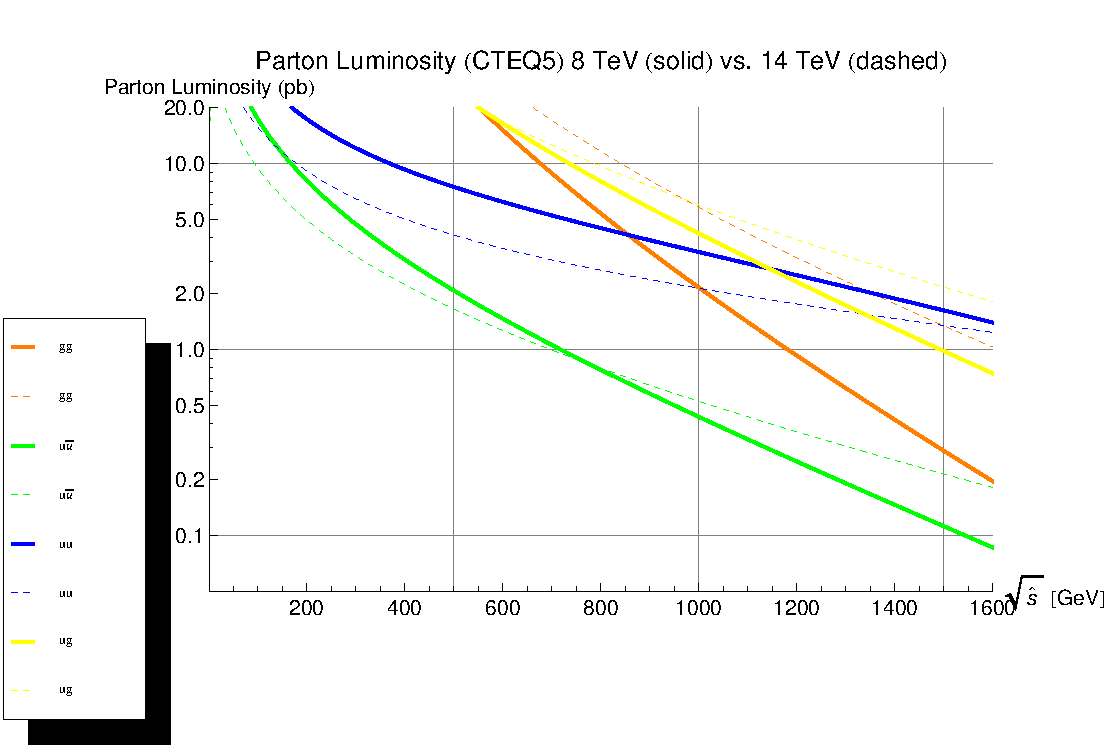
\includegraphics[width=.95\textwidth]{pics/parton_lumi_8TeV_14TeV}
\end{center}
\caption{Contours of the parton luminosity function derived from CTEQ5 parton distribution functions for $\sqrt{s}=8$ TeV and
$\sqrt{s}=14$ TeV. Contours are separated by collions the individual partons in the collision.  }
\label{fig:deltaRcones}
\end{figure}

Here the center term is refered to as the parton luminosity function and contains the parton distribution functions with
some extra accounting for the parton types to avoid double counting:
\begin{align*}
\tau\frac{dL_{ij}}{d\tau} = \frac{1}{1+\delta_{ij}} \int_0^1 dx_1 dx_2 \times \left [ (x_1 f_i(x_1,\mu^2) x_2 f_j(x_2,\mu^2)) + (1 \leftrightarrow 2)) \right ] \delta(\tau - x_1x_2) 
\end{align*}

\subsection{Kinematic Conventions for Collider Physics} 

\framebox{Pseudorapidity $\eta$} As the detector has cylindrical symmetry, the coordinate system used most
 commonly is two dimensional $(\eta, \phi)$. The pseudo-rapidity, $\eta$ is an approximation to rapidity, $y$, that is exact in the $\beta = 1$ limit:
\begin{align*}
y = \frac{1}{2}\log \frac{E - p_z}{E+p_z}\hspace{.75in} \eta = - \log \left( \tan\left (\frac{\theta}{2} \right ) \right)  
\end{align*}
where $\theta$ is the angle from the positive beam axis. This variable is useful for a number of reasons. 
Firstly, differences in rapidity are invariant under longitudinal lorrentz boosts along the beam axis. Also, 
for the energies being probed the particles in the decay products are of negligible mass and the approximation
 $\eta \approx y$ is nearly exact. Given this relation, pseudorapidity provides an intuitive geometric interpretation. 
Near full solid angle coverage is provided within $|\eta| < 5$

\begin{figure}
\begin{center}
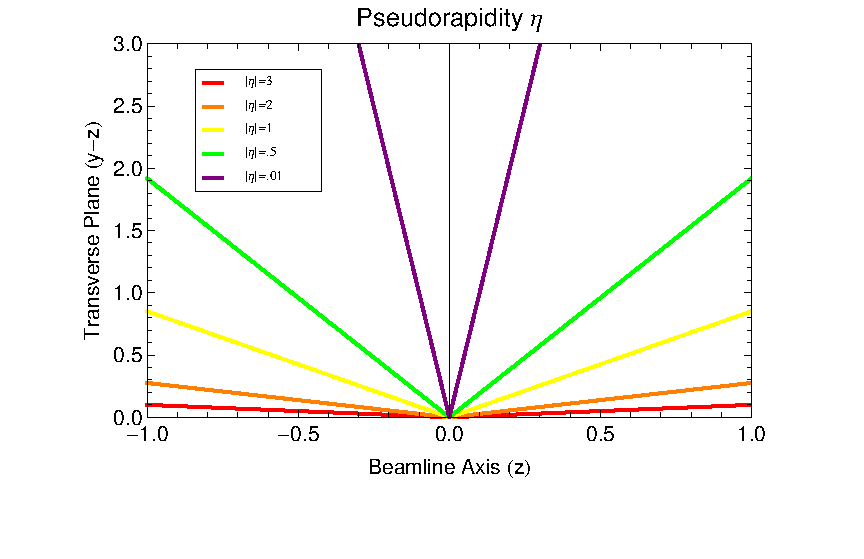
\includegraphics[width=.6\textwidth]{figures/exp_proj/pseudorapidity}
\end{center}
\caption{Lines of constant pseudorapidity in the z-y plane}
\label{fig:pseudorapidity}
\end{figure}

\framebox{$\Delta R$} Given our coordinate system, $\Delta R$ is our longitudinally boost invariant notion of distance:
\begin{align*}
\Delta R = \sqrt{ (\Delta \phi)^2 + (\Delta \eta)^2}
\end{align*}
Fixed values of $\Delta R$ form a solid angle ``cone'' extending from the interaction point outward. This can be seen by
 using our definition of $\eta$ to convert from cylindrical coordinates to $(x,y,z)$ and consider the distance relative to the point $(\eta_0,\phi_0)$
\begin{align*}
\Delta R = \sqrt{ \left( \phi_0 - \tan^{-1} (y/x) \right )^2 + \left ( \eta_0 + \log \left( \tan \frac{\cos^{-1} (z/\sqrt{x^2+y^2})}{2} \right) \right)^2 }
\end{align*}

\begin{figure}
\begin{center}
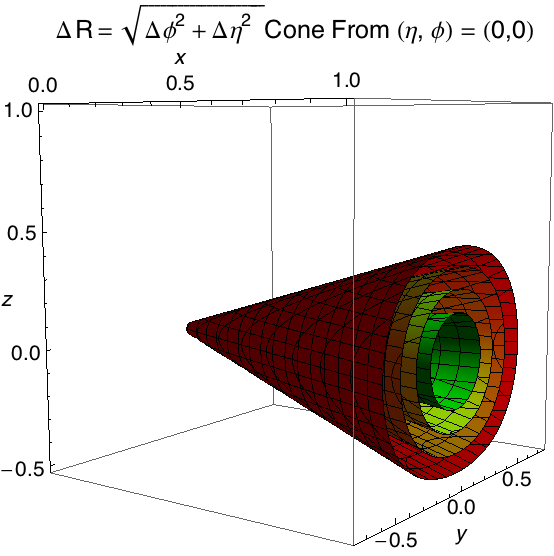
\includegraphics[width=.3\textwidth]{figures/exp_proj/deltaR_cone}
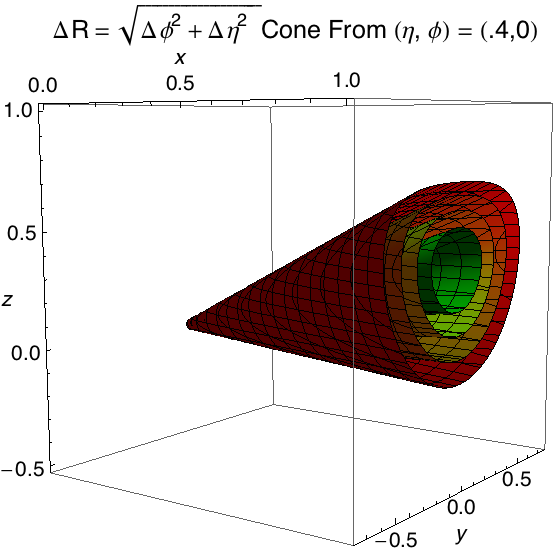
\includegraphics[width=.3\textwidth]{figures/exp_proj/deltaR_cone_eta0p4}
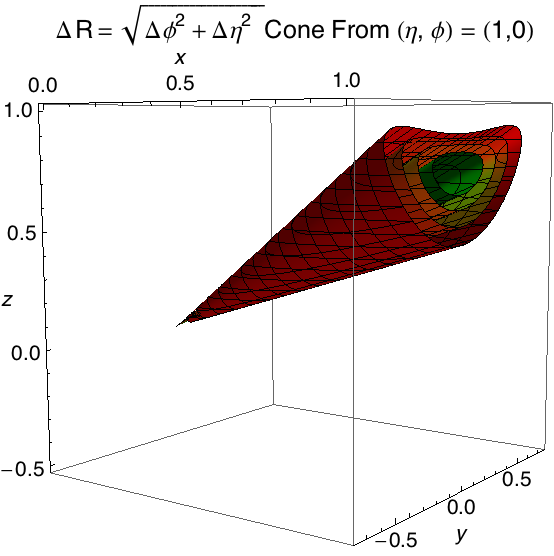
\includegraphics[width=.3\textwidth]{figures/exp_proj/deltaR_cone_eta1p0}
\end{center}
\caption{Contours of constant $\Delta R$ from the $\eta_),\phi_0 = 0,0$}
\label{fig:deltaRcones}
\end{figure}


\section{The Narrow Width Approximation}

\section{Event Simulation} 

\subsection{Hard Process Modeling}

\subsection{Parton Showering}

\subsection{Hadronization} 

$\Lambda_{QCD} \approx 0.1-0.3$ GeV 

top quark width is larger than lambda qcd and thus decays before hadronization. This allows for the study of a bare quark.
